%% Discover Artificial Intelligence (Springer Nature) manuscript, English version of the Japanese draft ver2
%% (paper/ja_v2/, 2026-11-17). Class: sn-jnl (copied once from the Springer Nature template on 2026-11-14).
%% Numbers are copied from the checked Japanese draft (each section of ja_v2 lists its sources in comments).
\documentclass[sn-nature,pdflatex]{sn-jnl}

\usepackage{amsmath,amssymb,amsfonts}
\usepackage{graphicx}
\usepackage{booktabs}
\usepackage{multirow}
\usepackage{xcolor}
\usepackage{array}
\usepackage{placeins}

% Draft markers (remove before submission).
\newcommand{\TBA}{\textcolor{red}{TBA}}
\newcommand{\PROV}[1]{\textcolor{orange}{#1}}  % value not yet re-checked
\newcommand{\pt}{\,points}

\begin{document}

\title[Few-label multimodal emotion recognition on a new corpus]{Multimodal emotion recognition on a new corpus with a few labels: which information sources correct which errors, when distillation helps, and emotion-wise reliability-weighted pseudo-labels}

\author*[1]{\fnm{TODO} \sur{TODO}}\email{TODO}

\affil*[1]{\orgdiv{TODO}, \orgname{TODO}, \orgaddress{\city{TODO}, \country{Japan}}}

\abstract{Multimodal emotion recognition (MER) classifiers have been reported to degrade on unseen corpora, and labelling a new corpus is costly. With few labels in a new corpus, unlabelled utterances, other labelled corpora and the other modalities of each utterance can help, but which of them corrects which classifier errors is unclear. Using linear classifiers on frozen audio, visual and text encoders, we split their error into a bias of predictions towards some emotions and the remaining error. Firstly, the audio and visual bias was almost removed without labels with one training corpus, whereas with all other corpora, pseudo-labels from classifiers including other modalities reduced the remaining error in nearly half of the conditions, and same-modality unlabelled utterances rarely did. Retraining audio classifiers on such pseudo-labels gave higher unweighted average recall (UAR) on all four test corpora. UAR rose only with pseudo-labels more accurate than the classifier before retraining. Secondly, as the most accurate modality varied by corpus and emotion, we propose late fusion that weights the audio, visual and text classifiers by strengths measured on the few labels and per-emotion profiles from other corpora, for more accurate pseudo-labels. On AFEW, IEMOCAP, MOSEI and MELD, also used to design it, the method had higher UAR than the equal-weight product of their probabilities in 11 of 12 conditions (5, 10, 25 labels per emotion; 2.1--3.5 points on AFEW). These findings suggest using unlabelled multimodal recordings for retraining and a few labels for weighting the modalities on a new corpus.}

\keywords{Multimodal emotion recognition, Cross-corpus transfer, Semi-supervised domain adaptation, Few labels, Pseudo-labels, Distillation, Late fusion}

\maketitle

% English version of paper/ja_v3/01_序論.md (ver3 draft 2, 2026-11-17). Structure of Ishii et al. 2022: field -> prior work -> However -> this study -> research questions and Fig. 1 -> "First, we analyze ... Second, we propose ... This method is motivated by ..." -> section guide. No contribution list (the research questions play that role; Ishii 2022). The scoped novelty statement is in Sect. 2.5 and the conclusion.
\section{Introduction}\label{sec:intro}

Multimodal emotion recognition (MER) estimates a speaker's emotion from the voice, face and words of the same utterance. Emotion corpora differ in environmental noise, recording devices, acted versus natural elicitation and speaker demographics \cite{gideon2021addog}, and also in how they were annotated. Emotion classifiers trained on one corpus have been reported to perform worse on other corpora \cite{ryumina2025,gideon2021addog}. Many methods for fusing modalities have been proposed, including for sentiment polarity \cite{zadeh2017tfn,mittal2020m3er,yu2021selfmm,yun2024telme}, and they have been evaluated by training and testing within one corpus; Ryumina et al.\ \cite{ryumina2025} noted that 12 recent methods evaluated on IEMOCAP, MOSEI, MELD or AFEW had not been evaluated across corpora. Using MER on utterances of a corpus not used for training requires adapting the classifiers to that corpus (the target).

Labels of naturally expressed emotions are collected from several raters who watch or listen to each utterance, which is costly to repeat for every new corpus \cite{parthasarathy2020ladder,abdelwahab2018dann}, whereas unlabelled utterances are easy to collect \cite{abdelwahab2018dann}. Adapting classifiers with labelled utterances of other corpora (sources) and unlabelled target utterances or a few target labels has mainly been studied for speech emotion recognition \cite{abdelwahab2018dann,gideon2021addog,feng2023}. The multimodal cross-corpus evaluations of Ryumina et al.\ \cite{ryumina2025} and Lian et al.\ \cite{lian2026merbench} did not use target labels, and He et al.\ \cite{he2025m4ser}, who addressed a setting with a few target labels, used audio and transcribed words. In MER, the other modalities of the same utterance can also be used as information attached to unlabelled utterances. Albanie et al.\ \cite{albanie2018} attached the predictions of a facial classifier to unlabelled videos and trained an audio emotion classifier towards them, and Zhang et al.\ \cite{zhang2021combining} combined training towards targets that include predictions of other modalities with semi-supervised learning. We call the four-emotion probabilities that classifiers including other modalities assign to unlabelled utterances \emph{pseudo-labels}, and retraining a classifier towards them without temperature \emph{distillation} \cite{hinton2015distilling,albanie2018}.

However, whether these findings hold in cross-corpus MER with only a few target labels per emotion is unknown. First, studies using sources and unlabelled utterances have compared the performance of methods, but which part of the classifier error these information sources and the other modalities correct has not been measured separately in one setting. Second, Albanie et al.\ and Zhang et al.\ did not evaluate this setting, so which classifiers distillation improves, and when, is unknown. Third, audio and visual classifiers have been reported to recognise different emotions well within one corpus \cite{busso2004}, but whether this holds when classifiers trained on source corpora are applied to a target, and if so how much weight each of the audio, visual and text classifiers should receive when their predictions are combined, has not been reported.

We consider a target with only K labels per emotion. The data available in this case, which we call information sources, are labelled source utterances, the K target labels, unlabelled target utterances and the other modalities of the same utterance; the first three form the setting of semi-supervised domain adaptation \cite{saito2019mme}. We place linear emotion classifiers on features of frozen pretrained audio, visual and text encoders and split their error into the part where predictions are biased towards some emotions (\emph{answer bias}) and the part that remains after removing that bias (\emph{remaining error}). Linear classifiers on frozen features serve as a setting for measuring what each information source changes in a classifier, not as a proposed classifier architecture, and we do not claim that the results hold for fine-tuned encoders (Sect.~\ref{sec:limitations}). We answer three research questions (Fig.~\ref{fig:questions}).
\begin{itemize}
\item \textbf{RQ1(a):} Does each of the four information sources correct the answer bias or the remaining error?
\item \textbf{RQ1(b):} Does distillation raise the UAR of the audio, visual and text classifiers and of the classifier on their concatenated features (AVT)? Which classifiers gain, and when?
\item \textbf{RQ2:} How should the predictions of the audio, visual and text classifiers be combined to raise the UAR of the pseudo-labels?
\end{itemize}

\begin{figure}[t]
\centering
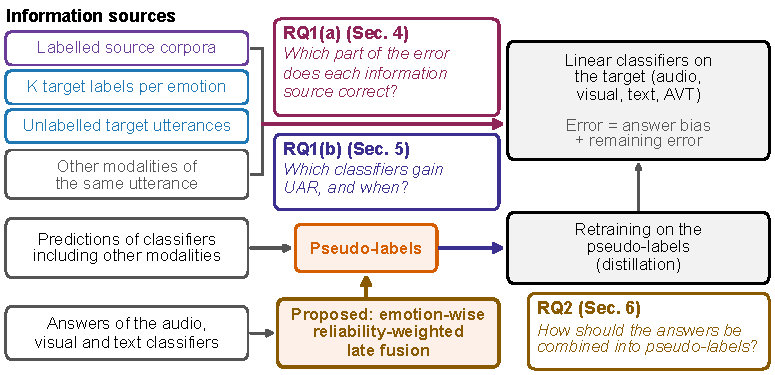
\includegraphics[width=\textwidth]{figures/fig_v2_questions_en.pdf}
\caption{The three research questions, written on the arrows of the processing flow they ask about}\label{fig:questions}
\end{figure}

First, we analyse in three settings with different numbers of source corpora which part of the error each information source reduces, to address RQ1(a) and RQ1(b) (Sect.~\ref{sec:analysis}). For audio classifiers with one source corpus (K = 5), label-free feature-mean subtraction obtained 4.69\pt\ of the 5.26-point gain of training on the source and the K labels together. With all non-target corpora as sources, the remaining error was reduced in 7 of 210 conditions by eight methods that use same-modality unlabelled utterances and in 38 of 81 conditions by distillation on pseudo-labels including other modalities. With each of AFEW, IEMOCAP (improvised), MOSEI and MELD in turn as the target, distillation gave higher audio UAR in all 12 conditions (K = 5, 10, 25; 1.4--4.1\pt\ in point estimates), and every pseudo-label with which UAR rose had higher UAR than the classifier before retraining. Second, we propose late fusion that measures each classifier's strength on the K target labels and its per-emotion profile on the source corpora, to address RQ2 (Sects.~\ref{sec:method} and \ref{sec:experiments}). This method aims to raise the UAR of the pseudo-labels with weights that differ by classifier and emotion, in line with the analysis result above and with the finding that the strongest modality differed by corpus (the order in which the method was designed is given in Sect.~\ref{sec:idea}). The proposal had higher UAR than the product of the three classifiers' probabilities in 11 of 12 conditions in point estimates, by 2.1--3.5\pt\ on AFEW.

Section~\ref{sec:related} reviews related work and Sect.~\ref{sec:setup} describes the data, features, classifiers, the three settings and the list of compared conditions. Section~\ref{sec:analysis} presents the analysis for RQ1(a) and RQ1(b), Sect.~\ref{sec:method} the method for RQ2 and Sect.~\ref{sec:experiments} its experiments. Section~\ref{sec:discussion} discusses the answer to each question against prior work, Sect.~\ref{sec:limitations} states limitations and Sect.~\ref{sec:conclusion} concludes.

% English version of paper/ja_v2/02_関連研究.md (2026-11-17).
\section{Related work}\label{sec:related}

\subsection{Semi-supervised domain adaptation}
Methods usable in semi-supervised domain adaptation, in which the target has a few labels, have been proposed for each information source: learning representations that do not reveal the domain (domain-adversarial neural networks, DANN) \cite{ganin2016dann} and aligning feature covariances (CORAL) \cite{sun2016coral} for unlabelled targets, entropy minimisation and pseudo-labels from semi-supervised learning \cite{grandvalet2004,lee2013pseudolabel}, and minimax entropy (MME) for semi-supervised domain adaptation \cite{saito2019mme}. Adding source data can also lower target performance (negative transfer) \cite{wang2019negative}. The method studies above compare methods that combine information sources and do not measure, in one setting, which part of the classifier error each source corrects.

\subsection{Cross-corpus MER with few labels}\label{sec:rel-cc}
For audio emotion classifiers that degrade on another corpus, adversarial learning that aligns representations with unlabelled target utterances \cite{abdelwahab2018dann} and learning that pulls together representations learned per corpus \cite{gideon2021addog} have been proposed. Ryumina et al.\ \cite{ryumina2025} evaluated the four corpora of our leave-one-corpus-out setting (IEMOCAP, MOSEI, MELD and AFEW; we use only the improvised part of IEMOCAP) with four emotions without target labels and showed that training on several corpora raised UAR by 1.7--6.6\pt. Lian et al.\ \cite{lian2026merbench} built cross-corpus benchmarks with shallow classifiers on frozen features and reported that multimodal models exceeded unimodal ones by small differences across corpora. For targets with a few labels, Feng and Chaspari \cite{feng2023} proposed metric learning for audio features, Li et al.\ \cite{li2021acted} adaptation of audio and video between acted and improvised speech, and He et al.\ \cite{he2025m4ser} a method using audio and speech-recognition transcripts.

\subsection{Distillation from other modalities}\label{sec:rel-distill}
Albanie et al.\ \cite{albanie2018} attached facial-expression predictions to unlabelled videos and trained an audio emotion classifier on them, and Zhang et al.\ \cite{zhang2021combining} combined this scheme with semi-supervised learning. Transferring representations or predictions of one modality to a model of another through paired unlabelled data is also used outside emotion recognition \cite{gupta2016,jaritz2020xmuda}. Training on the predictions of a more accurate model of another modality has been reported not to always improve the trained model \cite{xue2023mfh}.

\subsection{Late fusion and reliability weights}\label{sec:rel-fusion}
Zadeh et al.\ \cite{zadeh2017tfn} criticised late fusion, which trains unimodal classifiers separately and combines their predictions, for not learning interactions between modalities because it assumes that simple weighted averaging is a proper fusion approach. Predictions can be combined by product or sum rules \cite{kittler1998}. Busso et al.\ \cite{busso2004} reported that modality strengths differ by emotion, Kaya et al.\ \cite{kaya2017} chose model-by-emotion weights on AFEW by random search on validation data, M3ER \cite{mittal2020m3er} learned a multiplicative fusion layer that strengthens reliable modality cues per utterance, and Mar\'in et al.\ \cite{marin2026classwise} used per-utterance, per-emotion modality weights output by a network trained with all labels within one corpus.

\subsection{Position of this study}\label{sec:position}
% ver3: rewritten after reviews/v2_ja/prose_intro (Sect. 3) and citations_intro (16--18).
This study examines distillation in a setting that belongs to both the cross-corpus MER of Sect.~\ref{sec:rel-cc} and the distillation from other modalities of Sect.~\ref{sec:rel-distill}: cross-corpus MER with only a few target labels per emotion. Unlike Albanie et al., who used only facial predictions, our pseudo-labels are built from three classifiers including text. To the best of our knowledge, no prior study has compared, for the audio classifier under the same conditions, distillation on pseudo-labels including other modalities with 11 domain adaptation, semi-supervised and test-time adaptation methods that do not use such pseudo-labels (Sect.~\ref{sec:compmethods}; versions moved to linear classifiers on frozen features) in cross-corpus MER with audio, visual and text and only a few target labels per emotion. Three comparisons are close. Zhang et al.\ (2021) \cite{zhang2021combining} compared pseudo-labels including facial predictions with same-modality semi-supervised learning for speech emotion recognition, but used all training labels of the evaluated corpus (IEMOCAP) and did not compare domain adaptation methods. Jaritz et al.\ \cite{jaritz2023xmossda} compared cross-modal learning with uni-modal unsupervised domain adaptation methods moved to a semi-supervised setting, but for 3D semantic segmentation. Zhang et al.\ (2024) \cite{zhang2024amanda} proposed a multimodal domain adaptation method that uses no target labels (Amanda) between IEMOCAP, MELD, MOSEI and MSP-IMPROV and compared it with DANN and other domain adaptation methods, but not with distillation on pseudo-labels from other modalities.

Multimodal models trained on few samples can fall below the best unimodal model \cite{huang2021}. In RQ2 we use late fusion (Sect.~\ref{sec:rel-fusion}) to combine predictions into pseudo-labels. Unlike M3ER and Mar\'in et al., which learn per-utterance weights, the proposal uses one weight per classifier and emotion. To our knowledge, splitting a reliability table into classifier strengths measured on the K target labels and per-emotion profiles measured on the source corpora has not been reported.

% English version of paper/ja_v2/03_共通の設定.md (2026-11-17).
% ver3 draft 2 (2026-11-17): Table 1 gains the LOCO column (per-emotion LOCO counts moved to Table S1), the settings figure moved to Fig. S1, and Sect. 3.6 adds the numbered list of compared conditions (Table 2; the form of Table 1 and conditions (1)--(14) of Ishii et al. 2022), as in paper/ja_v3/03_データと設定.md.
\section{Data, features, classifiers and compared conditions}\label{sec:setup}

This section describes the data, features, classifiers, metric and three settings shared by all analyses and experiments, and lists the compared conditions.

\subsection{Corpora and four emotions}
We use six corpora that differ in elicitation, recording and annotation as seven groups (Table~\ref{tab:corpora}). IEMOCAP \cite{busso2008iemocap} is split into improvised and scripted groups, because in scripted sessions ten actors read the same lines and a text classifier could succeed by memorising them. The leave-one-corpus-out (LOCO) setting (Sect.~\ref{sec:settings}) uses the four corpora with audio, visual and text (AFEW, the improvised part of IEMOCAP, MOSEI and MELD), and the RQ2 evaluation adds CREMA-D (audio and visual). Labels are mapped to Neutral, Happy, Sad and Angry \cite{ryumina2025}, and utterances of other emotions are not used. In IEMOCAP, happy and excited are merged into Happy and frustration is not mapped to Angry. In MOSEI, an utterance with exactly one emotion of intensity at least 0.5 receives that emotion, one with none receives Neutral, and one with two or more is not used, so MOSEI Neutral is not a neutral rating by annotators.

\begin{table}[t]
\caption{The seven groups. Speaker and utterance counts are after restricting to four emotions, for the single-source and all-source settings; utterance and per-emotion counts are for the audio (WavLM) set, with differing visual or text counts in parentheses. The last column gives, for the LOCO setting (utterances with audio, visual and text; CREMA-D: audio and visual), the utterances, the clusters used to form test folds and their effective number $(\sum_g n_g)^2/\sum_g n_g^2$ for cluster sizes $n_g$; per-emotion LOCO counts are in Table~S1. Mod.: modalities. All corpora are in English (RAVDESS: North American English)}\label{tab:corpora}
\footnotesize\setlength{\tabcolsep}{3pt}
\begin{tabular}{@{}p{1.55cm}p{1.7cm}p{1.95cm}p{0.75cm}r p{1.5cm}p{1.7cm}p{1.35cm}@{}}
\toprule
Group & Elicitation & Annotation & Mod. & Speakers & Utterances & N / H / S / A & LOCO (clusters, effective) \\
\midrule
AFEW \cite{dhall2012afew,dhall2013emotiw} & Movie acting (partly natural) & Facial-expression category by raters & A, V, T$^{b}$ & 282$^{a}$ & 795 & 207 / 213 / 178 / 197 & 790 (51, 14.99) \\
IEMOCAP impro.\ \cite{busso2008iemocap} & Improvised acting & Plurality of raters' categories & A, V, T & 10 & 2,943 & 1,099 / 947 / 608 / 289 & 2,943 (5, 4.91) \\
IEMOCAP script.\ \cite{busso2008iemocap} & Scripted acting & Same & A, V, T & 10 & 2,588 (V 2,549) & 609 / 689 / 476 / 814 & -- \\
MOSEI \cite{zadeh2018mosei} & None (opinion monologues) & Crowd intensities of six emotions; our rule & A, V, T & 2,626$^{c}$ & 18,919 (V 18,634) & 8,847 / 6,790 / 1,830 / 1,452 & 18,634 (2,614, 783.22) \\
MELD \cite{poria2019meld} & TV-series acting & Majority of raters' categories & A, V, T & 283 & 11,343 (V 11,308, T 11,344) & 6,430 / 2,305 / 1,002 / 1,606 & 11,267 (272, 8.59) \\
CREMA-D \cite{cao2014cremad} & Instructed acting, 12 sentences & Acted emotion; crowd ratings & A, V & 91 & 4,900 (V 4,899) & 1,087 / 1,271 / 1,271 / 1,271 & 4,899 (91, 90.98) \\
RAVDESS \cite{livingstone2018ravdess} & Instructed acting, 2 sentences & Acted emotion; validated by raters & A & 24 & 672 & 96 / 192 / 192 / 192 & -- \\
\botrule
\end{tabular}
\footnotetext{$^{a}$Number of actor names. $^{b}$AFEW text features come from Whisper large-v3 transcripts (790 utterances) and were made after the single-source and all-source computations, which therefore do not use them. $^{c}$Number of channels or video IDs (Sect.~\ref{sec:split}). The two IEMOCAP groups share the same ten actors. Concatenated features are built only from utterances that have all of the concatenated modalities. LOCO clusters: actor/movie links (AFEW), sessions (IEMOCAP), channels or videos (MOSEI), speakers (MELD, CREMA-D)}
\end{table}

\subsection{Speaker-independent splits}\label{sec:split}
In every setting, no speaker appears on both the training and the evaluation side (speaker-independent), and official splits are not used. MOSEI has no speaker annotation, so the YouTube channel (known for 1,122 of 3,225 videos) or otherwise the video ID serves as the speaker; the same person may therefore appear on both sides in different videos. In the LOCO setting, aliases of the same MELD actor are merged, speaker names that do not identify a single voice are dropped, and AFEW utterances linked by actor or by movie form one cluster.

\subsection{Features and classifiers}
Features are encoder outputs averaged within each utterance; no encoder is fine-tuned on our corpora. Audio: 16 kHz waveforms (first 60 s) are fed to WavLM-large \cite{chen2022wavlm} and the last layer is averaged over time (1,024 dimensions); in the single-source setting we also use the last layer of HuBERT-large \cite{hsu2021}. Visual: the largest face is cropped with YOLOv8n-face\footnote{https://github.com/derronqi/yolov8-face (GPL-3.0), trained on WIDER FACE \cite{yang2016}.} from 5--6 frames per second (for IEMOCAP, the half of the screen showing the speaker), and the 512-dimensional outputs of a ResNet-50 expression model \cite{ryumina2022} are averaged over frames. Text: transcripts are fed to RoBERTa-base \cite{liu2019roberta} and the last layer is averaged over tokens (768 dimensions); human transcripts are used for IEMOCAP, MOSEI and MELD and Whisper large-v3 \cite{radford2023whisper} outputs for AFEW. RAVDESS and CREMA-D have no text features because their sentences are fixed, and RAVDESS has no visual features. Classifiers on concatenated features of two or three modalities (AV, VT, AT, AVT) are also built. We write A for audio, V for visual and T for text.

Every classifier is a multinomial logistic regression trained on per-dimension standardised features. With $n$ training utterances and $n_k$ of emotion $k$, utterances of emotion $k$ are weighted by $\omega_k=n/(4n_k)$ so that the emotion proportions of the training data do not enter the classifier. In the single-source setting, the classifier weights carry an L2 penalty with inverse strength $C$ and the intercepts are unpenalised; $C\in\{0.01,0.1,1,10\}$ is chosen by speaker-split three-fold cross-validation (the merged classifier uses the $C$ of the source-only classifier of the same repetition). In the all-source and LOCO settings, the classifier weights and intercepts are pulled towards a classifier built from the sources (the \emph{anchor}) with strengths $C'$ and $C_b$, chosen with source groups or corpora as provisional targets (Sect.~\ref{sec:settings}). Test labels are never used to choose hyperparameters.

\subsection{Three settings}\label{sec:settings}
The three settings differ in how labelled source utterances are used, and each provides the comparisons needed by one question (Fig.~S1). The single-source setting separates what one source corpus and the K labels correct (RQ1(a)); the all-source setting uses all groups as sources and compares the information sources that reduce the remaining error (RQ1(a)); the LOCO setting treats each corpus in turn as the new corpus to evaluate distillation and the proposal (RQ1(b), RQ2).
\begin{itemize}
\item \textbf{Single-source setting}: for each ordered pair of groups (target, source), all utterances of one source group and K target labels are trained together (merged classifier); classifiers trained on the source only and on the K target labels only are also built. The test set is one of five speaker folds of the target, and repetitions 0--9 change the folds and the test fold.
\item \textbf{All-source setting}: a classifier built from all groups except the target is the anchor and is retrained on the K target labels (K-label baseline), with K = 0, 5 and 25.
\item \textbf{LOCO setting}: one of AFEW, IEMOCAP (improvised), MOSEI and MELD is the target and the other three are sources. The mean of the weights and intercepts of the three source classifiers is the anchor, and the classifier retrained from it on the K target labels is the \emph{K-label baseline} (at K = 0, the anchor itself, i.e., source only). The test set is one of five folds that keep each cluster within one fold (one session for IEMOCAP), and the remaining target utterances are the \emph{candidates}; K labels per emotion are drawn from the candidates and no other candidate labels are used. Values are averaged over 50 repetitions (5 folds $\times$ 10 draws of the K labels; 5 repetitions for K = 0).
\end{itemize}

LOCO hyperparameters were selected on runs in which each of the three corpora other than the evaluation target served in turn as a provisional target (with the remaining two corpora as sources; 3 corpora $\times$ 5 folds $\times$ 2 seeds = 30 repetitions) and fixed, and the evaluation target was computed once with the fixed settings (evaluation run). We call each provisional-target computation an \emph{episode}. Outputs inspected before and during the evaluation run are stated in Sects.~\ref{sec:rq1b-compare} and \ref{sec:hp}.

\subsection{Metric and intervals}
The main metric is UAR (unweighted average recall over emotions), whose chance level with four emotions is 25\%. Overall accuracy (weighted accuracy) is not reported because it depends on the share of Neutral, which differs across corpora. UAR and its differences are in percentage points, and the difference A $-$ B between two classifiers is called the \emph{gain}; each section states A and B. All intervals are 95\% intervals without multiple-comparison correction; they reflect the sampling of test speakers (clusters for MOSEI and the LOCO setting) and of the K labels, not the choice of source corpora, training utterances, methods or hyperparameters. Intervals of the single-source and all-source settings are described in Sect.~\ref{sec:rq1a-compare}. For the LOCO setting, the variance of a cluster jackknife (cluster resampling for MOSEI and CREMA-D) is added to the variance over K-label draws; because inference with few clusters is anti-conservative \cite{cameron2008}, jackknife $t$ intervals are used for corpora with fewer than 20 effective test clusters. Conditions of the same corpus that differ only in K share test utterances and nested K labels and are not independent. We write that UAR \emph{rose} or \emph{fell} only when the 95\% interval of the difference lies above or below zero, and write ``higher in point estimates'' otherwise.

\subsection{Compared conditions}\label{sec:conditions}
Table~\ref{tab:conditions} lists the compared conditions with numbers that run consecutively within each comparison group. Condition 0 of each group ((A0), (B0), (C0), (D0), (E0)) is the starting point of the group (the source-only classifier, the K-label baseline or the product), and conditions of one group use the same test utterances in the same repetitions; groups D and E are reported as differences from the proposal, (D4) and (E2). Group D compares \emph{estimation-time decisions}: the argmax of the combined predictions of the three classifiers on test utterances, without retraining any classifier. Groups A and B serve RQ1(a) (Sect.~\ref{sec:rq1a-compare}), group C serves RQ1(b) (Sect.~\ref{sec:rq1b-compare}), and groups D and E serve RQ2 (Sect.~\ref{sec:compare}); each of these sections states what each comparison verifies. In the information-source columns, ``Source'' is labelled source utterances (including the anchor built from them in the all-source and LOCO settings), ``K'' the K target labels, ``Unl.'' unlabelled target utterances and ``Other'' features or predictions of a modality other than that of the classifier being retrained.

\begin{table}[!htbp]
\caption{Compared conditions. \checkmark: the condition uses the information source; --: it does not}\label{tab:conditions}
\footnotesize\setlength{\tabcolsep}{3pt}
\begin{tabular}{@{}l p{6.3cm} cccc@{}}
\toprule
No. & Condition & Source & K & Unl. & Other \\
\midrule
\multicolumn{6}{@{}p{12.6cm}@{}}{\textbf{A: single-source setting} (ordered pairs of the 7 groups, K = 5; (A1) K = 1, 5, 10)} \\
(A0) & Source-only classifier & \checkmark & -- & -- & -- \\
(A1) & Target-only classifier & -- & \checkmark & -- & -- \\
(A2) & Merged classifier (all source utterances and the K labels trained together) & \checkmark & \checkmark & -- & -- \\
(A3) & Intercept-only fix (weights of (A0) fixed; only intercepts learned on the K labels) & \checkmark & \checkmark & -- & -- \\
(A4) & Mean subtraction (the mean of all utterances is subtracted from source and target features before retraining) & \checkmark & -- & \checkmark$^{a}$ & -- \\
(A5) & Intercepts corrected on the K labels after mean subtraction & \checkmark & \checkmark & \checkmark$^{a}$ & -- \\
\multicolumn{6}{@{}p{12.6cm}@{}}{\textbf{B: all-source setting} (K = 0, 5, 25; (B2)--(B9) K = 0, 5)} \\
(B0) & K-label baseline (anchor retrained on the K labels) & \checkmark & \checkmark & -- & -- \\
(B1) & Distillation (retrained on pseudo-labels from classifiers including other modalities) & \checkmark & \checkmark & \checkmark & \checkmark \\
(B2)--(B9) & Eight methods that use same-modality unlabelled utterances$^{b}$ & \checkmark & \checkmark & \checkmark & -- \\
\multicolumn{6}{@{}p{12.6cm}@{}}{\textbf{C: LOCO setting} (AFEW, IEMOCAP, MOSEI, MELD; K = 0, 5, 10, 25; (C2)--(C12) K = 5, 10, 25; (C13) K = 5, 25)} \\
(C0) & K-label baseline (audio, visual, text, AVT) & \checkmark & \checkmark & -- & -- \\
(C1) & Distillation (retrained on the product pseudo-labels) & \checkmark & \checkmark & \checkmark & \checkmark \\
(C2)--(C11) & Ten methods that use no information from other modalities$^{c}$ & \checkmark & \checkmark & \checkmark$^{c}$ & -- \\
(C12) & xMUDA-style mutual mimicry between unimodal classifiers (no pseudo-labels including other modalities)$^{c}$ & \checkmark & \checkmark & \checkmark & \checkmark \\
(C13) & Retraining with other pseudo-label providers (360 variants per K) & \checkmark & \checkmark & \checkmark & \checkmark\ or --$^{d}$ \\
\multicolumn{6}{@{}p{12.6cm}@{}}{\textbf{D: LOCO setting, estimation-time decisions} (K = 5, 10, 25; CREMA-D in the SI)} \\
(D0) & Product (of the probabilities of the three classifiers that make the pseudo-labels of (C1)) & \checkmark & \checkmark & \checkmark & \checkmark \\
(D1) & Probability mean (sum rule) & \checkmark & \checkmark & \checkmark & \checkmark \\
(D2) & Per-classifier temperature calibration (fitted by log-likelihood on the K labels) & \checkmark & \checkmark & \checkmark & \checkmark \\
(D3) & Decisions of the single classifier strongest on the K labels & \checkmark & \checkmark & \checkmark & \checkmark \\
(D4) & Proposal (Sect.~\ref{sec:method}) & \checkmark & \checkmark & \checkmark & \checkmark \\
(D5) & Proposal without per-emotion profiles & \checkmark & \checkmark & \checkmark & \checkmark \\
(D6) & Proposal without strength differences & \checkmark & \checkmark & \checkmark & \checkmark \\
\multicolumn{6}{@{}p{12.6cm}@{}}{\textbf{E: LOCO setting, retrained AVT} (K = 5, 10, 25)} \\
(E0) & K-label baseline AVT (the AVT of (C0)) & \checkmark & \checkmark & -- & -- \\
(E1) & AVT retrained on the product pseudo-labels (the AVT of (C1)) & \checkmark & \checkmark & \checkmark & \checkmark \\
(E2) & AVT retrained on the proposal's pseudo-labels & \checkmark & \checkmark & \checkmark & \checkmark \\
\botrule
\end{tabular}
\footnotetext{$^{a}$The target mean is taken over all target utterances including the test utterances; no labels are used. $^{b}$(B2) entropy minimisation, (B3) self-training, (B4) IM, (B5) T3A, (B6) label propagation, (B7) CORAL, (B8) DANN, (B9) MME. $^{c}$(C2) self-training, (C3) entropy minimisation, (C4) IM, (C5) T3A, (C6) label propagation, (C7) pseudo-labels from the retrained classifier's own (C0) probabilities, (C8) training on labelled source utterances and the K labels together (S+T), (C9) CORAL, (C10) DANN, (C11) MME, (C12) xMUDA-style. (C8)--(C11) also train on the source utterances themselves, and (C8) uses no unlabelled target utterances. (C2)--(C12) are the 11 methods that do not use pseudo-labels including other modalities; (C12) was computed only for the audio, visual and text classifiers. For group D, ``Other'' means that predictions of the three modalities are combined; the single classifier of (D3) was retrained on the probabilities of the AVT classifier (Sect.~\ref{sec:rq1b-compare}). $^{d}$Depending on the provider, the pseudo-labels do or do not include predictions of other modalities (providers listed in Sect.~\ref{sec:rq1b-compare})}
\end{table}

% English version of paper/ja_v3/04_解析.md (ver3 draft 2, 2026-11-17). The former RQ1(a) and RQ1(b) sections are merged into one analysis section (Ishii et al. 2022): a comparison subsection per question (what each numbered comparison verifies), then a results subsection whose subheadings name the comparisons and whose last paragraph gives the answer in one sentence. Interpretation and links to prior work are in the Discussion. The two-errors, distillation-flow and advantage figures and the table of the 11 methods moved to the Supplementary Information.
\FloatBarrier
\section{Analysis: which errors the information sources reduce, and when distillation raises UAR}\label{sec:analysis}

This section compares the conditions of groups A--C (Sect.~\ref{sec:conditions}) to analyse which part of the error each of the four information sources corrects (RQ1(a)) and which classifiers distillation improves, and when (RQ1(b)).

\subsection{Two parts of the error}\label{sec:twoerrors}
A linear classifier assigns an emotion using, for each pair of emotions, a boundary in feature space whose direction is set by the weights and whose position is set by the intercepts (Fig.~S2). An error in which the boundary has the right direction but is shifted, so that predictions are biased towards one emotion, is the \emph{answer bias}; it disappears when only the intercepts are corrected. The error that remains after correcting the bias is the \emph{remaining error}; it shrinks only when the direction of the weights changes.

We quantify the two parts as follows. For the score $s_k(x)=w_k^\top x+b_k$ of emotion $k$, the decision between emotions $k$ and $l$ is the sign of $z_{kl}=(w_k-w_l)^\top x+(b_k-b_l)$. With mean $\hat\mu_k$ and variance $v_k$ of $z_{kl}$ over target test utterances of emotion $k$ (likewise for $l$) and $\sigma=\sqrt{(v_k+v_l)/2}$, we define
\begin{equation}
d_{kl}=\frac{\hat\mu_k-\hat\mu_l}{\sigma},\qquad o_{kl}=-\frac{\hat\mu_k+\hat\mu_l}{2\sigma},
\end{equation}
the separation of the two emotions on the decision axis and the offset of the boundary ($z_{kl}=0$) from the midpoint of their means. If $z_{kl}$ of both emotions is normal with equal variance, the pairwise accuracy is $A(d,o)=\tfrac12[\Phi(d/2-o)+\Phi(d/2+o)]$. With the separation $D^{*}$ along the linear discriminant direction of the labelled target utterances (Ledoit--Wolf shrinkage \cite{ledoit2004}), the pairwise loss splits as
\begin{equation}
A(D^{*},0)-A(d,o)=\underbrace{[A(D^{*},0)-A(d,0)]}_{\text{direction loss}}+\underbrace{[A(d,0)-A(d,o)]}_{\text{intercept loss}}.
\end{equation}
Changing only the intercepts shifts $z_{kl}$ equally for all utterances and moves only $o$; a shift $x\to x+\delta$ common to all emotions also moves only $o$, so subtracting each corpus's feature mean does not change the direction loss. $D^{*}$ is used only for evaluation and is not the largest separation over linear directions. When this equal-variance Gaussian approximation was checked on source-only classifiers of the single-source setting, it met the pre-set fit criterion (median approximation error below one third of the median loss) for the direction loss except for visual features, but not for the intercept loss (Supplementary Information S2), so answer bias is measured by UAR differences rather than by the approximation.

\subsection{Comparisons for RQ1(a)}\label{sec:rq1a-compare}
In group A (single-source setting, K = 5), the following comparisons separate what one source corpus and the K labels correct.
\begin{itemize}
\item \textbf{(A2) $-$ (A0):} the gain of adding the K labels to the source-only classifier (hereafter the merged gain).
\item \textbf{(A3) $-$ (A0) and (A4) $-$ (A0):} neither the intercept-only fix nor mean subtraction changes the direction loss (Sect.~\ref{sec:twoerrors}); the share of the merged gain that they obtain measures how much correcting answer bias alone obtains.
\item \textbf{(A5) $-$ (A4):} whether correcting intercepts on the K labels adds to mean subtraction.
\item \textbf{The ratio $d_T(K)/D^{*}$ of (A1)} (K = 1, 5, 10): how close the weight direction comes to that of $D^{*}$ when only the K labels are used (remaining error).
\end{itemize}
In group B (all-source setting), we measure whether (B1) and each of (B2)--(B9) reduce the direction loss, averaged over the six emotion pairs, relative to (B0). The provider and weighting of the pseudo-labels of (B1) were chosen per condition on provisional targets (mostly the product of the classifiers' probabilities), and all include the retrained classifier's own modality. (B1) is measured in 81 conditions (each classifier with audio, visual and text on three corpora and with audio and visual on five corpora; K = 0, 5, 25) and (B2)--(B9) in 210 conditions (single modality; K = 0, 5), so the two counts do not compare the same conditions. Pre-set rules classified each condition as \emph{reduced}, \emph{same level}, \emph{increased} or \emph{undetermined} from the 95\% interval of the direction-loss difference ((B0) $-$ method) and an equivalence margin $\delta$ set from provisional-target outputs only (the full rules, the values of $\delta$, the hyperparameter selection and the intervals of groups A and B are in Supplementary Information S2). Some pseudo-label options (such as the product) were added after seeing results of an earlier version of the method on the same corpora.

\subsection{Results for RQ1(a)}

\subsubsection{Group A: the six conditions of the single-source setting}\label{sec:rq1a-single}
Table~\ref{tab:rq1a}(a) shows the group A differences by feature set. For audio and visual features, the intercept-only fix (A3) and mean subtraction (A4) obtained most of the merged gain. The summed (A3) gain was 0.78--0.91 times the summed merged gain. Label-free (A4) gained 4.69\pt\ [3.81, 5.57] for audio (WavLM) against the merged 5.26\pt, and 2.40\pt\ for visual against 2.47\pt. The interval of (A5) $-$ (A4) was not above zero for any of the eight feature sets (two audio, visual, text and four concatenations).

For (A1), which uses no source, $d_T/D^{*}$ (median over targets of the ratio averaged over six emotion pairs) was 0.23, 0.47 and 0.62 for audio (WavLM) at K = 1, 5 and 10, and 0.11, 0.32 and 0.42 for text. Visual reached 1.01 at K = 10 (the ratio can exceed 1 because $D^{*}$ is not the largest linear separation).

\begin{table}[!htbp]
\caption{Results for RQ1(a). (a) Group A (single-source setting, K = 5): UAR differences in points on test utterances; values are pair means (each pair averaged over repetitions 0--9); ``Ratio'' is $\sum$((A3) $-$ (A0)) $/ \sum$((A2) $-$ (A0)) over pairs; the last column gives 95\% intervals. (b) Group B (all-source setting): numbers of conditions by verdict. Direction loss: reduced / same level / increased / undetermined; UAR (method $-$ (B0)): higher / same level / lower / undetermined. ``16 more'' are conditions in which the adaptation term of DANN or MME did not change predictions beyond seed variation (separate from the 48 undetermined). Visual direction losses come from features that failed the approximation check (Sect.~\ref{sec:twoerrors})}\label{tab:rq1a}
\footnotesize
\textit{(a) Group A}\par\smallskip
\begin{tabular}{@{}lrrrl@{}}
\toprule
Features & (A2) $-$ (A0) & (A4) $-$ (A0) & Ratio & (A5) $-$ (A4) \\
\midrule
Audio (WavLM) & +5.26 & +4.69 & 0.91 & +0.38 [$-$0.12, +0.88] \\
Audio (HuBERT) & +4.73 & +4.18 & 0.90 & +0.18 [$-$0.42, +0.77] \\
Visual & +2.47 & +2.40 & 0.78 & $-$0.39 [$-$0.78, +0.02] \\
\botrule
\end{tabular}\par\medskip
\textit{(b) Group B}\par\smallskip
\begin{tabular}{@{}lllrll@{}}
\toprule
Cond. & Modalities & Classifier & Conditions & Direction loss$^{a}$ & UAR \\
\midrule
(B1) & A, V, T (3 corpora) & Audio & 9 & 9/0/0/0 & 9/0/0/0 \\
 &  & Visual & 9 & 1/1/0/7 & 1/0/0/8 \\
 &  & Text & 9 & 5/0/1/3 & 4/0/0/5 \\
 &  & AVT & 9 & 6/1/0/2 & 5/2/0/2 \\
 & A, V (5 corpora) & Audio & 15 & 7/0/0/8 & 7/0/0/8 \\
 &  & Visual & 15 & 5/0/0/10 & 4/1/0/10 \\
 &  & AV & 15 & 5/5/0/5 & 2/2/0/11 \\
\midrule
(B1) total & & & 81 & 38/7/1/35 & 32/5/0/44 \\
(B2)--(B9) & Single modality & A, V, T & 210 & 7/60/79/48 (16 more) & --- \\
\botrule
\end{tabular}
\footnotetext{$^{a}$Halving $\delta$ gives 49 of 81 ``reduced'' conditions for (B1); doubling it gives 20}

\end{table}

\subsubsection{Group B: (B1) and (B2)--(B9) in the all-source setting}\label{sec:rq1a-all}
Table~\ref{tab:rq1a}(b) shows that (B1) reduced the direction loss in 38 of 81 conditions and increased it in one; its UAR was judged higher than (B0) (same rule) in 32 and lower in none. (B2)--(B9) reduced the direction loss in 7 of 210 conditions and increased it in 79. If the true differences were zero and conditions independent, the expected numbers of ``reduced'' conditions would be 2.02 and 5.25. Comparing point estimates on the same anchors and conditions (two modality groups, K = 0 and 5), (B1) reduced the direction loss more in 341 of 373 pairs (pairs are not independent).

\subsubsection{Summary of the results for RQ1(a)}
The answer to RQ1(a) is therefore as follows. With one source corpus, the K labels and the source mainly corrected answer bias for audio and visual features, and label-free mean subtraction almost corrected it as well. In the all-source setting, pseudo-labels including other modalities reduced the remaining error in 38 of 81 conditions, whereas same-modality unlabelled utterances reduced it in only 7 of 210.

\subsection{Comparisons for RQ1(b)}\label{sec:rq1b-compare}
Distillation (C1) in group C (LOCO setting) retrains each of the audio, visual and text classifiers and the AVT classifier. The pseudo-label $q_i$ of each candidate utterance is the \emph{product}: the audio, visual and text classifiers are retrained from the anchor on the K labels and on the probabilities that the AVT classifier of (C0) assigns to the candidates, and their three probabilities are multiplied per utterance and normalised (Fig.~S3). $q_i$ includes the prediction of the retrained classifier's own modality. The loss of the retrained linear classifier is the cross-entropy on the K labels plus the cross-entropy towards the pseudo-labels of the candidates (the pseudo-label probabilities are targets without temperature) plus L2 terms towards the anchor $(W_0,b_0)$:
\begin{equation}
\begin{split}
L(W,b)=\frac{1}{S}\Big[&a\sum_{i\in\mathcal{K}}-\log p(y_i\mid x_i)+\sum_{i\in\mathcal{U}}\sum_k g_{ik}\,(-\log p(k\mid x_i))\\
&+\frac{\|W-W_0\|^2}{2C'}+\frac{\|b-b_0\|^2}{2C_b}\Big],
\end{split}
\end{equation}
with $p(\cdot\mid x)=\mathrm{softmax}(Wx+b)$ and $g_{ik}=(\rho n/4)\,q_{ik}/\sum_{j\in\mathcal{U}}q_{jk}$, where $\mathcal{K}$ is the set of K labelled utterances, $\mathcal{U}$ is the set of all $n$ candidates (including $\mathcal{K}$) and $S$ is the sum of the loss weights. The pseudo-label weights sum to $\rho n/4$ for each emotion. This loss form was fixed before the evaluation run; five other loss forms, including the temperature loss of Albanie et al.\ \cite{hinton2015distilling,albanie2018}, are compared in Supplementary Information S4. $C'$ and $C_b$ are those of (C0); the pseudo-label weight $\rho$, the K-label multiplier $a$ and the exponents of each modality in the product were chosen on the mean UAR over provisional targets (Sect.~\ref{sec:settings}); when several points were within two standard errors of the best, the one closest to the untuned values ($\rho=1$, $a=1$, exponents (1, 1, 1)) was chosen (grids in Supplementary Information S4). In all 48 conditions with K = 5, 10 and 25, the selected values gave the same classifier as the untuned values, so the product of (C1) and (D0) multiplies the three probabilities with equal weights. The values were fixed and recorded in a version-controlled file before the single evaluation run. The authors inspected UARs and differences (without intervals) of (C1) and (C2)--(C12) during the evaluation run (AFEW, IEMOCAP) and before aggregation; aggregation scripts were fixed beforehand and not changed.

Group C provides three comparisons.
\begin{itemize}
\item \textbf{(C1) $-$ (C0)} (audio, visual, text, AVT; K = 0, 5, 10, 25): which classifiers distillation improves.
\item \textbf{(C1) $-$ (C2)--(C12)} (K = 5, 10, 25): whether the gain of distillation can be obtained without pseudo-labels including other modalities. The 11 methods start from the same anchor and K labels and select hyperparameters by the same procedure. Because the encoders are frozen, DANN and MME are versions with their loss terms on a linear map and classifier, not the original methods that also train the feature extractor.
\item \textbf{Advantage and gain in (C13)} (K = 5, 25): how the gain of distillation relates to how often the pseudo-labels are correct.
\end{itemize}

(C13) consists of the retraining runs in which the evaluation run retrained each of the four classifiers on predictions of other classifiers instead of the product, with untuned $\rho=1$ and $a=1$. The providers are classifiers of (C0) (unimodal classifiers of other modalities, classifiers on two concatenated modalities, AVT), the product, the three classifiers that make the product, the AVT anchor and the classifiers of each source corpus. For each variant we measure (Fig.~S4):
\begin{itemize}
\item the \emph{advantage}: UAR of the provider's decisions $-$ UAR of the classifier before retraining, (C0), on candidates excluding the K labels, using candidate labels that are never used for retraining;
\item the \emph{gain}: UAR of the retrained classifier $-$ UAR of (C0) on test utterances.
\end{itemize}
K is 5 and 25, for which the candidate decisions of (C0) were saved. Excluding AVT retrained on its own predictions and duplicates of other providers leaves 360 variants per K (the excluded variants are in Supplementary Information S2; one of them, whose advantage is zero by construction, had a gain interval above zero). This is a descriptive analysis set up after the computation, without prior predictions; the authors had seen the gains and intervals of some providers before setting it up. Variants share candidates, test utterances and pseudo-label ingredients, so the rank correlations and counts below are not tests.

\subsection{Results for RQ1(b)}

\subsubsection{(C1) $-$ (C0): gain of distillation}\label{sec:rq1b-audio}
Table~\ref{tab:gain} shows (C1) $-$ (C0). Audio UAR after distillation was higher than that of (C0) in all 12 conditions with K = 5, 10 and 25 in point estimates, with intervals above zero in the nine conditions other than IEMOCAP (+2.71 to +4.15\pt). IEMOCAP gained +1.45 to +2.41\pt\ with intervals including zero at all three K. Without labels (K = 0), the audio gain had intervals above zero on all four corpora (+2.13 to +4.86\pt). The audio classifier retrained on pseudo-labels alone (K = 0) had higher UAR in point estimates than (C0) with 5 and 10 labels per emotion on all four corpora (values in Supplementary Information S2; no intervals computed).

The other classifiers gained less. Text gained +5.01 to +7.34\pt\ on IEMOCAP at K = 5, 10 and 25 with intervals above zero and had intervals including zero elsewhere; visual intervals were above zero only for MOSEI at K = 10 and 25, and AVT intervals only for MELD at all K and MOSEI at K = 25.

\begin{table}[!htbp]
\caption{(C1) $-$ (C0): gain of distillation (UAR points on test utterances) with 95\% intervals without correction. Values average 50 repetitions (5 for K = 0). At K = 0, (C0) is the anchor (source only) and (C1) uses no labels. K = 10 values follow an aggregation decided before the evaluation run (intervals only, no tests). IEMOCAP: improvised part}\label{tab:gain}
\footnotesize\setlength{\tabcolsep}{3.4pt}
\begin{tabular}{@{}lllll@{}}
\toprule
Corpus & K = 0 & K = 5 & K = 10 & K = 25 \\
\midrule
\multicolumn{5}{@{}l}{\textit{Audio}} \\
AFEW & +4.86 [+2.32, +7.40] & +4.15 [+2.56, +5.74] & +3.78 [+2.19, +5.38] & +3.32 [+1.40, +5.25] \\
IEMOCAP & +4.76 [+1.89, +7.63] & +2.41 [$-$0.45, +5.27] & +2.01 [$-$0.57, +4.58] & +1.45 [$-$0.48, +3.37] \\
MOSEI & +2.13 [+1.08, +3.19] & +3.19 [+2.38, +3.99] & +4.11 [+3.20, +5.01] & +3.36 [+2.56, +4.16] \\
MELD & +3.89 [+0.28, +7.51] & +3.12 [+1.18, +5.06] & +2.71 [+0.66, +4.77] & +2.86 [+1.21, +4.51] \\
\multicolumn{5}{@{}l}{\textit{Visual}} \\
AFEW & +2.48 [$-$1.34, +6.31] & +0.09 [$-$2.99, +3.17] & +0.18 [$-$1.90, +2.26] & $-$0.18 [$-$1.40, +1.04] \\
IEMOCAP & $-$2.08 [$-$5.19, +1.03] & $-$0.84 [$-$4.75, +3.06] & +0.91 [$-$4.76, +6.58] & $-$0.74 [$-$6.30, +4.82] \\
MOSEI & $-$0.91 [$-$2.35, +0.54] & +0.21 [$-$1.14, +1.56] & +1.56 [+0.16, +2.95] & +2.57 [+1.17, +3.98] \\
MELD & +0.67 [$-$2.76, +4.10] & +0.85 [$-$0.91, +2.61] & +0.71 [$-$0.50, +1.93] & +1.11 [$-$0.18, +2.40] \\
\multicolumn{5}{@{}l}{\textit{Text}} \\
AFEW & +1.56 [$-$2.33, +5.46] & +1.65 [$-$1.50, +4.79] & +1.83 [$-$0.92, +4.58] & +0.75 [$-$2.07, +3.56] \\
IEMOCAP & +7.52 [+4.75, +10.29] & +7.34 [+4.37, +10.31] & +6.87 [+3.06, +10.67] & +5.01 [+2.44, +7.57] \\
MOSEI & $-$0.69 [$-$1.72, +0.35] & $-$0.02 [$-$0.89, +0.84] & +0.79 [$-$0.02, +1.60] & +0.03 [$-$0.69, +0.74] \\
MELD & +0.18 [$-$2.56, +2.92] & $-$1.18 [$-$4.44, +2.08] & $-$1.28 [$-$3.15, +0.59] & $-$0.94 [$-$2.84, +0.95] \\
\multicolumn{5}{@{}l}{\textit{AVT}} \\
AFEW & +1.69 [$-$1.91, +5.30] & +1.03 [$-$0.65, +2.72] & +1.10 [$-$0.44, +2.65] & +0.62 [$-$0.33, +1.57] \\
IEMOCAP & +1.65 [$-$2.86, +6.16] & +0.16 [$-$4.53, +4.85] & +0.24 [$-$3.62, +4.09] & $-$0.83 [$-$5.12, +3.46] \\
MOSEI & $-$0.32 [$-$1.17, +0.54] & $-$0.35 [$-$0.90, +0.19] & +0.17 [$-$0.37, +0.70] & +0.74 [+0.18, +1.30] \\
MELD & +3.36 [+0.90, +5.81] & +2.53 [+1.65, +3.42] & +1.87 [+0.94, +2.80] & +1.41 [+0.63, +2.19] \\
\botrule
\end{tabular}
\end{table}

\subsubsection{(C1) $-$ (C2)--(C12): the 11 other methods}\label{sec:rq1b-methods}
For audio, (C1) $-$ method was positive in point estimates in all 132 comparisons over K = 5, 10 and 25, with intervals not above zero only in 10 comparisons on IEMOCAP (K = 5 UARs in Table~S2). (C7), which uses the classifier's own (C0) probabilities as pseudo-labels, gave $-$1.0 to +0.5\pt\ relative to (C0). For AVT the differences were mixed: some methods, such as self-training (C2) on AFEW (72.1 vs 70.8), were higher than (C1) in point estimates, and at K = 5 only CORAL (C9) on MOSEI was higher than (C1) with the interval of the difference below zero. The 11 methods use information other than pseudo-labels including other modalities, so we read these differences as differences in the information used rather than in the quality of the methods.

\subsubsection{(C13): advantage and gain}\label{sec:rq1b-margin}
For example, on MOSEI with K = 25, retraining the audio classifier on pseudo-labels from the visual--text classifier gave an advantage of +4.6\pt\ (42.2 vs 37.6) and a gain of +2.05 [+0.74, +3.35]\pt. On AFEW with K = 5, retraining the visual classifier on pseudo-labels from the audio--text classifier gave an advantage of $-$16.7\pt\ (54.4 vs 71.1) and a gain of $-$4.40 [$-$7.70, $-$1.09]\pt.

Over the 360 variants, the ranks of advantage and gain agreed: the rank correlation was 0.80 at K = 5 and 0.83 at K = 25, and within each of the 32 combinations of corpus, retrained classifier and K it was positive (median 0.92, minimum 0.39). Figure~\ref{fig:margincounts} counts the variants by the sign of the advantage and the gain interval. No variant with a negative advantage (173 at K = 5, 184 at K = 25) had a gain interval above zero, and 125 and 144 had intervals below zero. Among variants with a positive advantage (187 and 176), 58 and 42 had intervals above zero, while 16 and 20 had intervals below zero (breakdown in Supplementary Information S2).

\begin{figure}[t]
\centering
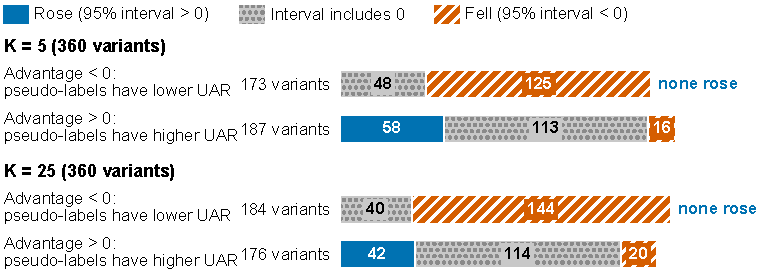
\includegraphics[width=\textwidth]{figures/fig_margin_counts_en.pdf}
\caption{Variants of (C13) (360 per K; K = 5 and 25) counted by the sign of the advantage and by the 95\% interval of the gain (above zero, including zero, below zero). One variant is one combination of corpus, retrained classifier and pseudo-label provider; the gain is the difference in test UAR. No variant with a negative advantage rose}\label{fig:margincounts}
\end{figure}

Among unimodal classifiers, the one whose (C0) had the highest candidate UAR (hereafter the corpus's strongest modality) was visual on AFEW, audio on IEMOCAP, visual on MOSEI and text on MELD at both K = 5 and 25. Retraining the classifier of the strongest modality on pseudo-labels from the classifier on the concatenated features of the other two modalities gave negative gains in point estimates in all eight cases (four corpora and two K; $-$4.40 to $-$1.02\pt).

\subsubsection{Summary of the results for RQ1(b)}
The answer to RQ1(b) is therefore as follows. Distillation gave higher audio UAR than (C0) in all 12 conditions in point estimates, with intervals above zero in the nine conditions other than IEMOCAP, and the gains of the visual, text and AVT classifiers varied in sign across corpora. Every (C13) variant whose UAR rose had pseudo-labels with higher UAR than the classifier before retraining.

% English version of paper/ja_v3/05_手法.md (ver3 draft 2, 2026-11-17). Following Ishii et al. 2022, the method section opens with the motivation, linking each analysis result to one design decision, and states the scope ("Our goal is not ... but ...") before the definition. The weight-table decomposition and episode figures moved to the Supplementary Information (Figs. S7, S8); the AFEW evaluation-run values moved to Sect. 6.3.
\FloatBarrier
\section{Method: emotion-wise reliability-weighted late fusion}\label{sec:method}

\subsection{Motivation}\label{sec:idea}
The idea of the proposal was conceived after seeing outputs of the evaluation run of distillation in Sect.~\ref{sec:analysis}, and its form was fixed on provisional-target computations (Sect.~\ref{sec:hp}); the (C13) aggregation of Sect.~\ref{sec:rq1b-margin} was set up after the method had been fixed. Below we state the three design decisions and the results that correspond to each.

First, the goal of the method is to raise the UAR of the pseudo-labels. In the (C13) aggregation set up later, every variant whose UAR rose also had pseudo-labels with higher UAR than the classifier before retraining, and none of the 173 and 184 variants with a negative advantage rose (Sect.~\ref{sec:rq1b-margin}).

Second, the weights differ by classifier and emotion, whereas the pseudo-labels of distillation, (D0), multiply the three classifiers' probabilities with equal weights. In provisional-target computations run to design the method (Sect.~\ref{sec:settings}; each of the four corpora as a provisional target with two of the remaining corpora as sources, 30 repetitions each), the classifier-by-emotion reliabilities (Sect.~\ref{sec:method-def}) measured with all candidate labels were highest for visual on all four emotions of AFEW and for text on all four of MELD, for visual on Happy and audio on the others in IEMOCAP, and changed with the emotion in MOSEI (Fig.~\ref{fig:idea}). We therefore use 12 weights, one per classifier and emotion. In the (C13) aggregation set up later, the corpus's strongest modality also differed across corpora (visual on AFEW, audio on IEMOCAP, visual on MOSEI, text on MELD), and retraining the classifier of the strongest modality on pseudo-labels from the other two modalities gave negative gains in point estimates in all eight cases (Sect.~\ref{sec:rq1b-margin}).

\begin{figure}[t]
\centering
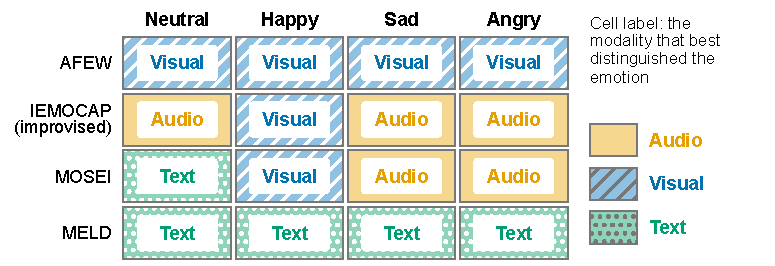
\includegraphics[width=\textwidth]{figures/fig_prop_idea_en.pdf}
\caption{For each corpus and emotion, the modality with the highest reliability. Values are reliabilities used to design the method (provisional-target computations, all candidate labels, K = 5, mean of 30 repetitions), not values of the evaluation run}\label{fig:idea}
\end{figure}

Third, measuring all 12 weights on the K target labels would determine each weight from only K utterances per emotion. In the same provisional-target computations, we built two classifier-by-emotion reliability tables, one measured on the sources and one on all candidate labels of the provisional target, and found that splitting the weights into two parts allows each part to be measured on different data (values in Supplementary Information S5). The ranking of classifier strengths (mean reliability over the four emotions) changed across corpora. For every corpus and K, the strongest modality by source-measured strength differed from that on all candidate labels in more than half of the repetitions, and the K-label strengths agreed in more repetitions than the source-measured ones in 11 of the 12 combinations of corpus and K. The classifier-by-emotion component left after removing classifier effects, emotion effects and a non-additivity term, by contrast, correlated positively between the source table and the candidate-label table. We therefore measure strengths on the K target labels and per-emotion profiles on the labelled source corpora.

Our goal is not to build a new fusion architecture that learns per-utterance weights, but to set, with only a few target labels, weights that raise the UAR of the pseudo-labels while fitting only three quantities (one strength per classifier) on the K labels.

\subsection{Definition}\label{sec:method-def}
The proposal weights the predictions of the classifiers that make the product of (C1) (the product components) with a classifier-by-emotion reliability table and turns the fused predictions into pseudo-labels. The table is the sum of strengths and per-emotion profiles (Fig.~S7).

The reliability is defined on the scores of each classifier. With probabilities $p_m(i\mid x)$ of classifier $m$ for emotion $i$, the centred log-probability is the score $z_m(i\mid x)=\log p_m(i\mid x)-\frac14\sum_j\log p_m(j\mid x)$, and
\begin{equation}\label{eq:rel}
d_m(i)=\max\!\big(0,\sqrt2\,\Phi^{-1}(A_m(i))\big),\quad A_m(i)\in[0.02,0.98],
\end{equation}
where $A_m(i)$ is the mean over emotions $j\neq i$ of the area under the ROC curve (AUC) separating utterances of true emotion $i$ from those of $j$ by $z_m(i\mid\cdot)$, and $\Phi^{-1}$ is the standard normal quantile function ($d_m(i)\le 2.90$). Because the ranks of scores do not change when intercepts are shifted, $d_m(i)$ depends neither on the classifier's intercepts nor on the target's emotion proportions. The mean over the four emotions is the strength $L_m$, and $d_m(i)-L_m$ is the per-emotion profile.

The strengths are measured on the K labels. The K labels are split into five subsets per emotion; for each subset $f$, the product components are retrained by the procedure of (C1) on the K labels without subset $f$ and assign probabilities to subset $f$; the reliabilities of Eq.~(\ref{eq:rel}) computed from the five subsets' probabilities are averaged over emotions to give $L^{K}_m$. Because $L^{K}_m$ is noisy for small K, a default strength $L^{0}_m$ (the mean of the three $L^{K}_m$ or the strength measured on the sources) is mixed in with weight $n_0$:
\begin{equation}
L_m=\frac{n\,L^{K}_m+n_0\,L^{0}_m}{n+n_0},\qquad n=4K.
\end{equation}

The profiles are measured on the source corpora. Within each source $s$, $d^{\mathrm{in}}_{s,m}(i)$ is measured by speaker-split five-fold cross-validation, and a classifier trained on all of $s$ is applied to another source $t$ to give $d^{\mathrm{out}}_{s\to t,m}(i)$. The share of modality $m$'s reliability that carries over to other corpora is $\eta_m=\sum_{s\to t}\sum_i d^{\mathrm{out}}_{s\to t,m}(i)/\sum_{s\to t}\sum_i d^{\mathrm{in}}_{s,m}(i)$ (clipped to $[0,1.5]$), and
\begin{equation}
d^{\mathrm{src}}_m(i)=\eta_m\frac{1}{|S|}\sum_s d^{\mathrm{in}}_{s,m}(i),\qquad r^{\mathrm{src}}_m(i)=d^{\mathrm{src}}_m(i)-\frac14\sum_j d^{\mathrm{src}}_m(j)
\end{equation}

The reliability table combines strengths and profiles, and the fused predictions give the pseudo-labels. The table is $T(m,i)=\max(0,L_m+\beta\,r^{\mathrm{src}}_m(i))$ ($\beta=1$ uses the profiles, $\beta=0$ does not); dividing by its mean gives weights $\Omega(m,i)=T(m,i)/(\frac{1}{12}\sum_{m',i'}T(m',i'))$, and the scores are summed per emotion, $s(i\mid x)=\sum_m \Omega(m,i)\,z_m(i\mid x)$. Because emotion-specific weights can shift predictions towards some emotions, intercepts $c$ are shifted without labels so that the mean of $\mathrm{softmax}(s(\cdot\mid x)+c)$ over candidates equals the mean of the product's probabilities (fixed-point iteration). The fused decision at estimation time is $\arg\max_i(s(i\mid x)+c_i)$. We attach $q(i\mid x)=\mathrm{softmax}_i(s(i\mid x)+c_i)$ to the candidates as pseudo-labels (soft labels) and retrain the AVT classifier (AV for CREMA-D) with the loss of (C1) (Sect.~\ref{sec:rq1b-compare}). Because the fused predictions carry information of all three modalities, the retrained classifier is AVT, which takes all three features; comparisons of estimation-time decisions (group D) do not depend on it. Audio, visual and text classifiers retrained on the proposal's pseudo-labels were not computed (Sect.~\ref{sec:limitations}). $\rho$ and $a$ are borrowed from the values chosen for the product's pseudo-labels.

\subsection{Hyperparameter selection on source-corpus episodes}\label{sec:hp}
The hyperparameters ($n_0\in\{0,20,80,\infty\}$, $\beta\in\{0,1\}$ and the two default strengths; 16 settings, 14 distinct) were selected, per evaluation target and K, by the highest mean UAR on the test folds of the provisional targets over three episodes in which each source corpus served in turn as a provisional target with the other two as sources (3 corpora $\times$ 5 folds $\times$ 2 seeds = 30 repetitions; Fig.~S8). No data of the evaluation target enter any episode. All selected settings had $\beta=1$, and $n_0$ was 0 in 8 of 12 conditions and 20 in the other four. The setting $n_0=\infty$, $\beta=0$ with the mean default strength gives the same decisions as the product. For CREMA-D, the hyperparameters ($n_0=0$, $\beta=1$) and $\rho$ and $a$ for the AV classifier were selected on the repetitions of a six-corpus provisional-target computation (the four corpora plus CREMA-D and RAVDESS) that do not involve CREMA-D. The form of the method was fixed after seeing the provisional-target runs, and the evaluation was computed once; the idea of the proposal was conceived after seeing outputs of the evaluation run of (C1)--(C13), and CREMA-D was added to the evaluation after its values had been seen in the six-corpus provisional runs (Sect.~\ref{sec:limitations}).

% English version of paper/ja_v3/06_実験.md (ver3 draft 2, 2026-11-17). Ishii et al. 2022 form: method -> comparisons (what each numbered comparison verifies) -> results (subheadings name the comparisons; table reading, one paragraph per comparison, a summary paragraph with the answer in one sentence). Tables 8 and 9 of draft 1 are merged into Table 5; the comparator table moved to Table S3. Counts not in draft 1 ((D4) - (D1): 8 of 12, 4 above zero; (E2) - (E0): 10 of 12, 7 above zero) were counted from the values of Table 5.
\FloatBarrier
\section{Experiments: evaluation of the proposal}\label{sec:experiments}

\subsection{Procedure}\label{sec:procedure}
The evaluation targets are AFEW, IEMOCAP (improvised), MOSEI and MELD, with K = 5, 10 and 25 and 50 repetitions (5 folds $\times$ 10 draws). K labels, candidates, test utterances and product components are those of the (C1) evaluation run; only the classifiers measuring strengths and the AVT retrained on the proposal's pseudo-labels, (E2), are new. The proposal needs K labels, so there is no K = 0 condition. Intervals are those of the LOCO setting (Sect.~\ref{sec:setup}). CREMA-D (audio and visual) is also evaluated with 50 repetitions and four source corpora (Supplementary Information S7).

\subsection{Comparisons}\label{sec:compare}
Group D compares the estimation-time decisions of conditions that use the same product components and K labels and differ only in how predictions are combined; these comparisons do not depend on the retrained classifier. Group E compares the UAR of retrained AVT classifiers.
\begin{itemize}
\item \textbf{(D4) $-$ (D0), (D1):} the product and sum rules \cite{kittler1998} combine the three classifiers with equal weights and use no K labels. This verifies whether classifier-by-emotion weights raise UAR.
\item \textbf{(D4) $-$ (D2):} (D2) fits per-classifier inverse temperatures to the K-label log-likelihood (temperature scaling \cite{guo2017calibration}); like the proposal, it fits three quantities on the K labels.
\item \textbf{(D4) $-$ (D3):} (D3) selects the product component with the highest K-label strength and uses its decisions. This verifies whether combining the three classifiers itself raises UAR. (D3) was added after the evaluation run from its saved outputs (outside the evaluation protocol), with the same label-free intercept shift as the proposal.
\item \textbf{(D4) $-$ (D5), (D6):} (D5) sets $\beta=0$ and (D6) replaces the three strengths by their K-label mean. These verify the contributions of the per-emotion profiles and the strength differences.
\item \textbf{(E2) $-$ (E0), (E1):} whether the AVT retrained on the proposal's pseudo-labels has higher UAR than the AVT before retraining and the AVT retrained on the product's pseudo-labels.
\end{itemize}
Comparisons with three further comparators that fit weights on the K labels and with four further combinations of the same predictions are in Supplementary Information S6, and the content and references of all comparators are in Table~S3.

\subsection{Results}\label{sec:rq2-results}
Table~\ref{tab:rq2} gives the UAR of groups D and E and the differences from the proposal. For each corpus, the upper rows are estimation-time decisions and the lower rows retrained AVT classifiers.

\begin{table}[!htbp]
\caption{Evaluation of the proposal: UAR (points, test utterances, mean of 50 repetitions). (D4): the proposal's estimation-time decisions; (E2): the AVT retrained on its pseudo-labels. Parentheses: (D4) $-$ row for group D and (E2) $-$ row for group E, with 95\% intervals without correction; rows (D5) and (D6) give only the difference. * interval above zero (proposal higher); $\dagger$ below zero (proposal lower). (D3) was added after the evaluation run. Row names abbreviate those of Table~\ref{tab:conditions} (Mean: probability mean; Temp.: temperature calibration; Strongest: the single classifier strongest on the K labels; No profile: without per-emotion profiles; Equal str.: without strength differences; K-label: the AVT of (C0); Product: the AVT retrained on the product's pseudo-labels). CREMA-D (audio and visual) is in Table~S6}\label{tab:rq2}
\footnotesize\setlength{\tabcolsep}{1pt}
\begin{tabular}{@{}llll@{}}
\toprule
Row & K = 5 & K = 10 & K = 25 \\
\midrule
\multicolumn{4}{@{}l}{\textbf{AFEW}} \\
(D4) Proposal & 71.36 & 74.39 & 76.58 \\
(D0) Product & 69.23 (+2.13 [+1.0, +3.3]*) & 70.88 (+3.51 [+1.5, +5.5]*) & 73.45 (+3.14 [+1.9, +4.4]*) \\
(D1) Mean & 69.22 (+2.14 [+1.0, +3.2]*) & 71.02 (+3.38 [+1.9, +4.9]*) & 72.85 (+3.73 [+2.5, +5.0]*) \\
(D2) Temp. & 74.30 ($-$2.94 [$-$5.6, $-$0.3]$\dagger$) & 74.84 ($-$0.45 [$-$1.5, +0.6]) & 76.31 (+0.27 [$-$0.6, +1.1]) \\
(D3) Strongest & 68.65 (+2.70 [$-$3.3, +8.7]) & 70.21 (+4.18 [$-$1.2, +9.6]) & 72.79 (+3.79 [$-$1.5, +9.1]) \\
(D5) No profile & +0.38 [+0.03, +0.7]* & +0.45 [$-$0.1, +1.0] & +0.36 [$-$0.2, +1.0] \\
(D6) Equal str. & +1.74 [+0.4, +3.1]* & +3.20 [+1.1, +5.3]* & +2.57 [+1.4, +3.7]* \\
(E2) Proposal & 71.78 & 74.61 & 77.05 \\
(E0) K-label & 69.74 (+2.04 [+0.5, +3.6]*) & 71.56 (+3.05 [+1.8, +4.3]*) & 75.22 (+1.83 [+0.9, +2.8]*) \\
(E1) Product & 70.77 (+1.01 [+0.2, +1.8]*) & 72.66 (+1.95 [+0.5, +3.4]*) & 75.84 (+1.21 [+0.4, +2.0]*) \\
\midrule
\multicolumn{4}{@{}l}{\textbf{IEMOCAP (improvised)}} \\
(D4) Proposal & 72.56 & 73.80 & 75.03 \\
(D0) Product & 72.07 (+0.49 [$-$0.2, +1.2]) & 73.37 (+0.43 [$-$0.2, +1.1]) & 74.53 (+0.50 [+0.01, +1.0]*) \\
(D1) Mean & 73.03 ($-$0.46 [$-$2.8, +1.9]) & 74.25 ($-$0.46 [$-$3.1, +2.2]) & 75.52 ($-$0.49 [$-$3.2, +2.2]) \\
(D2) Temp. & 71.69 (+0.87 [+0.5, +1.2]*) & 73.16 (+0.64 [$-$0.1, +1.4]) & 74.37 (+0.67 [$-$0.2, +1.6]) \\
(D3) Strongest & 67.05 (+5.52 [+1.3, +9.8]*) & 68.42 (+5.38 [$-$0.5, +11.2]) & 71.51 (+3.52 [$-$3.6, +10.7]) \\
(D5) No profile & +0.24 [+0.03, +0.5]* & +0.23 [$-$0.05, +0.5] & +0.20 [$-$0.1, +0.5] \\
(D6) Equal str. & +0.38 [$-$0.2, +1.0] & +0.06 [$-$0.6, +0.7] & +0.22 [$-$0.3, +0.7] \\
(E2) Proposal & 72.81 & 73.86 & 74.95 \\
(E0) K-label & 72.55 (+0.25 [$-$4.5, +5.0]) & 73.49 (+0.36 [$-$3.7, +4.4]) & 75.51 ($-$0.56 [$-$4.7, +3.6]) \\
(E1) Product & 72.71 (+0.10 [$-$0.6, +0.8]) & 73.73 (+0.13 [$-$0.3, +0.6]) & 74.68 (+0.27 [$-$0.1, +0.6]) \\
\midrule
\multicolumn{4}{@{}l}{\textbf{MOSEI}} \\
(D4) Proposal & 41.16 & 42.82 & 44.47 \\
(D0) Product & 40.97 (+0.19 [$-$0.2, +0.6]) & 42.53 (+0.29 [$-$0.03, +0.6]) & 44.07 (+0.40 [+0.1, +0.7]*) \\
(D1) Mean & 41.01 (+0.15 [$-$0.2, +0.5]) & 42.56 (+0.26 [$-$0.1, +0.6]) & 43.94 (+0.52 [+0.2, +0.9]*) \\
(D2) Temp. & 39.98 (+1.18 [+0.7, +1.6]*) & 42.14 (+0.69 [+0.3, +1.0]*) & 44.11 (+0.36 [+0.1, +0.6]*) \\
(D3) Strongest & 36.83 (+4.33 [+3.5, +5.2]*) & 37.92 (+4.90 [+4.1, +5.7]*) & 39.20 (+5.27 [+4.5, +6.0]*) \\
(D5) No profile & +0.73 [+0.5, +1.0]* & +0.62 [+0.4, +0.9]* & +0.51 [+0.3, +0.7]* \\
(D6) Equal str. & $-$0.42 [$-$0.7, $-$0.1]$\dagger$ & $-$0.35 [$-$0.6, $-$0.1]$\dagger$ & $-$0.07 [$-$0.2, +0.1] \\
(E2) Proposal & 41.20 & 42.84 & 44.44 \\
(E0) K-label & 41.46 ($-$0.26 [$-$0.8, +0.3]) & 42.39 (+0.45 [$-$0.2, +1.0]) & 43.35 (+1.09 [+0.5, +1.7]*) \\
(E1) Product & 41.10 (+0.10 [$-$0.2, +0.4]) & 42.56 (+0.28 [$-$0.01, +0.6]) & 44.09 (+0.35 [+0.1, +0.6]*) \\
\midrule
\multicolumn{4}{@{}l}{\textbf{MELD}} \\
(D4) Proposal & 50.05 & 50.68 & 52.95 \\
(D0) Product & 50.15 ($-$0.09 [$-$0.6, +0.4]) & 50.20 (+0.48 [+0.01, +1.0]*) & 52.12 (+0.83 [+0.2, +1.5]*) \\
(D1) Mean & 50.28 ($-$0.22 [$-$1.4, +0.9]) & 50.38 (+0.30 [$-$0.7, +1.3]) & 52.30 (+0.65 [$-$0.1, +1.4]) \\
(D2) Temp. & 50.85 ($-$0.80 [$-$1.7, +0.1]) & 51.24 ($-$0.56 [$-$1.5, +0.3]) & 52.91 (+0.04 [$-$0.5, +0.6]) \\
(D3) Strongest & 46.79 (+3.27 [+1.6, +4.9]*) & 47.39 (+3.29 [+1.5, +5.1]*) & 50.08 (+2.88 [+1.4, +4.4]*) \\
(D5) No profile & +0.10 [$-$0.4, +0.6] & +0.14 [$-$0.5, +0.7] & +0.15 [$-$0.1, +0.4] \\
(D6) Equal str. & $-$0.19 [$-$0.7, +0.4] & +0.40 [$-$0.05, +0.8] & +0.75 [$-$0.004, +1.5] \\
(E2) Proposal & 50.07 & 50.38 & 52.73 \\
(E0) K-label & 47.59 (+2.48 [+1.8, +3.2]*) & 48.26 (+2.12 [+1.4, +2.8]*) & 50.49 (+2.24 [+1.6, +2.9]*) \\
(E1) Product & 50.13 ($-$0.05 [$-$0.6, +0.5]) & 50.13 (+0.25 [$-$0.2, +0.7]) & 51.90 (+0.82 [+0.2, +1.5]*) \\
\botrule\end{tabular}
\end{table}

\subsubsection{(D4) $-$ (D0), (D1): equal-weight combination rules}\label{sec:rq2-rules}
The proposal (D4) minus the product (D0) was positive in 11 of 12 conditions in point estimates, with intervals excluding zero in seven (AFEW at all K, IEMOCAP and MOSEI at K = 25, MELD at K = 10 and 25). The largest differences were on AFEW (+2.13 to +3.51\pt). On AFEW, the visual product component had a UAR more than 17\pt\ above the audio and text components (K = 5: visual 70.70, audio 53.24, text 45.76), and the visual classifier alone was higher than the product at K = 5 and 10 in point estimates (70.70 vs 69.23 and 71.93 vs 70.88). In the nine conditions on IEMOCAP, MOSEI and MELD, (D4) $-$ (D0) ranged from $-$0.09 to +0.83\pt. The difference from the probability mean, (D4) $-$ (D1), was positive in 8 of 12 conditions in point estimates, with intervals above zero on AFEW at all K and on MOSEI at K = 25 and below zero in none.

\subsubsection{(D4) $-$ (D2): a comparator fitted on the K labels}\label{sec:rq2-temp}
The difference from per-classifier temperature calibration, (D4) $-$ (D2), was positive in 8 of 12 conditions in point estimates, and the proposal was lower with an interval excluding zero only on AFEW at K = 5 ($-$2.94 [$-$5.6, $-$0.3], 71.36 vs 74.30). Comparisons with seven further comparators are in Supplementary Information S6.

\subsubsection{(D4) $-$ (D3): selecting the strongest single classifier}\label{sec:rq2-single}
The proposal (D4) was higher than the decisions of the single classifier strongest on the K labels (D3) in all 12 conditions in point estimates (+2.70 to +5.52\pt), with intervals above zero in seven (IEMOCAP at K = 5, MOSEI and MELD at all K). (D3) on AFEW at K = 5 (68.65) was lower than the visual classifier alone (70.70) because it selected a non-visual classifier in 3 of 50 repetitions and its intercepts were shifted (69.25 before the shift); the shift lowered (D3) on AFEW by 0.44--0.65\pt, and without the shift for either method (D4) $-$ (D3) was +1.86 to +6.11\pt\ in all 12 conditions (intervals above zero in eight). By contrast, per-emotion recall of (D4) was lower than that of (D3) in point estimates for Happy on AFEW ($-$6.42 to $-$4.39\pt), Neutral on MELD ($-$4.32 to $-$2.74\pt) and Sad on IEMOCAP at K = 25 ($-$0.21\pt; no per-emotion intervals computed). Splitting this difference, (D0) $-$ (D3) (+2.04 to +5.02\pt; intervals above zero in 7 of 9) accounted for most of it on IEMOCAP, MOSEI and MELD, and (D4) $-$ (D0) on AFEW ((D0) $-$ (D3) +0.57 to +0.67\pt), suggesting that multiplying the three classifiers' predictions raised UAR over selecting one on IEMOCAP, MOSEI and MELD, and changing their weights did so on AFEW.

\subsubsection{(D4) $-$ (D5), (D6): versions with one part removed}\label{sec:rq2-ablation}
On MOSEI, the difference from the proposal without per-emotion profiles, (D4) $-$ (D5), had intervals above zero at all K (+0.51 to +0.73\pt), and so did CREMA-D (Supplementary Information S7). On AFEW, the difference from the proposal without strength differences, (D4) $-$ (D6), had intervals above zero at all K (+1.74 to +3.20\pt), accounting for most of AFEW's (D4) $-$ (D0) (+2.13 to +3.51\pt). Counted after the evaluation over its 50 repetitions, the classifier with the highest K-label strength was the classifier with the highest strength on all candidate labels (visual on AFEW, audio on IEMOCAP, text on MELD) in 0.70--1.00 of repetitions, whereas the classifier with the highest source-measured strength was a different classifier on all three corpora. On MOSEI, where the top two strengths were close, this fraction was 0.30--0.38 (values per corpus and K in Supplementary Information S5).

\subsubsection{(E2) $-$ (E0), (E1): retrained AVT}\label{sec:rq2-retrained}
The AVT retrained on the proposal's pseudo-labels (E2) had higher UAR than the AVT retrained on the product's pseudo-labels (E1) in 11 of 12 conditions in point estimates, with intervals above zero in five (AFEW at all K, MOSEI and MELD at K = 25); on AFEW the differences were +1.01, +1.95 and +1.21\pt, and on the other three corpora $-$0.05 to +0.82\pt. The difference from the AVT before retraining, (E2) $-$ (E0), was positive in 10 of 12 conditions in point estimates, with intervals above zero in seven. On CREMA-D (audio and visual), the estimation-time (D4) $-$ (D0) and the retrained AV (E2) $-$ (E1) were +0.31 to +0.63\pt\ with all six intervals excluding zero (Supplementary Information S7).

\subsubsection{Summary of the results for RQ2}
The answer to RQ2 is therefore as follows. Combining predictions with reliabilities whose strengths come from the K labels and per-emotion profiles from the sources gave estimation-time UAR higher than the equal-weight product in 11 of 12 conditions in point estimates (by 2.1--3.5\pt\ on AFEW), and the AVT retrained on the resulting pseudo-labels had higher UAR than the AVT retrained on the product's pseudo-labels in 11 of 12. Differences from temperature calibration on the K labels, (D2), varied in sign.

% English version of paper/ja_v3/07_考察.md (ver3 draft 2, 2026-11-17). One subsection per research question (the "Answer to Q1" form of Ishii et al. 2022): observation -> meaning -> agreement and difference with prior work. Text moved from draft 1 (Answer to RQ1(b), Answer to RQ2, Relation to prior work, Where to spend effort).
\FloatBarrier
\section{Discussion}\label{sec:discussion}

\subsection{Answer to RQ1(a): answer bias was almost corrected without labels, and the remaining error was reduced by pseudo-labels including other modalities}\label{sec:disc-rq1a}
With one source corpus, most of the gain of the source and the K labels for audio and visual features was also obtained by correcting only the intercepts or by label-free feature-mean subtraction (Sect.~\ref{sec:rq1a-single}). This suggests that, in this setting, most of what the source and the K labels added to UAR came from correcting answer bias, which unlabelled target utterances could also provide. In the all-source setting, the error that remained after removing the bias was reduced by pseudo-labels including other modalities but rarely by same-modality unlabelled utterances (Sect.~\ref{sec:rq1a-all}). The domain adaptation and semi-supervised learning studies of Sect.~\ref{sec:related} compared the performance of methods that combine information sources; our results show that, when the error is split into two parts in one setting, same-modality unlabelled utterances and pseudo-labels including other modalities corrected different parts. The answer-bias result is limited to the single-source setting (Sect.~\ref{sec:limitations}).

\subsection{Answer to RQ1(b): distillation gave higher audio UAR, and UAR rose only when the pseudo-labels had higher UAR than the classifier before retraining}\label{sec:disc-rq1b}
In cross-corpus MER with only a few labels per emotion, distillation gave higher audio UAR than the classifier before retraining in all 12 conditions in point estimates and was higher than the 11 methods that do not use pseudo-labels including other modalities in all 132 comparisons in point estimates (Sects.~\ref{sec:rq1b-audio} and \ref{sec:rq1b-methods}). This is in the same direction as Albanie et al.\ \cite{albanie2018}, who showed that audio emotion classifiers can be trained on facial predictions.

No variant with a negative advantage (173 and 184) rose, whereas among variants with a positive advantage UAR rose in only 58 of 187 and 42 of 176 (Sect.~\ref{sec:rq1b-margin}). Training on the predictions of a more accurate model of another modality has been reported not to always improve the trained model \cite{xue2023mfh}. Our results suggest that pseudo-labels having higher UAR than the classifier before retraining is a necessary, but not a sufficient, condition for distillation to raise UAR.

One possible explanation of the audio gains is that audio was not the strongest modality on the corpora other than IEMOCAP and the product's pseudo-labels had higher candidate UAR than the audio K-label baseline, and that audio features predicted the text classifier's decisions better than visual features did (Supplementary Information S3). The advantage analysis is descriptive and was set up after the computation, and the analysis of S3 fixed its decision rule before computing but did not measure its relation to the gains, so neither establishes the cause of the gains.

\subsection{Answer to RQ2: weights with strengths from the K labels and profiles from the sources made pseudo-labels with higher UAR than the product}\label{sec:disc-rq2}
The difference between the proposal's estimation-time decisions and the product was largest on AFEW, where the visual classifier's UAR exceeded the audio and text classifiers by more than 17\pt\ (Sect.~\ref{sec:rq2-rules}). One possible explanation is that the product combines the log-probabilities of the visual, audio and text classifiers with equal weights, whereas the proposal gave the visual classifier larger weights according to the K-label strengths (K = 5 mean weights over emotions: visual 1.17, audio 0.93, text 0.90). Removing the strength differences lowered UAR on AFEW, and removing the profiles lowered UAR on MOSEI, where the strongest modality changed with the emotion (Sect.~\ref{sec:rq2-ablation}). The emotion-dependent differences in modality strength that Busso et al.\ \cite{busso2004} reported within one corpus were also observed across our corpora, where the ranking of classifier strengths changed from corpus to corpus (Sect.~\ref{sec:idea}).

With few training samples, a model trained on more modalities has been argued to be able to fall below a model trained on a subset of them \cite{huang2021}. The proposal combines the decisions of three separately trained classifiers with three quantities set on the K labels; in this form, it was higher than the decisions of the single classifier strongest on the K labels in all 12 conditions in point estimates (a post hoc comparison; Sect.~\ref{sec:rq2-single}). Differences from temperature calibration on the K labels varied in sign (Sect.~\ref{sec:rq2-temp}), and differences from the product may be biased in favour of the proposal because the method was built on the evaluation corpora (Sect.~\ref{sec:limitations}).

\subsection{Where to spend effort on a new corpus}
The results inform whether to spend effort on labelling or on collecting unlabelled recordings for a new corpus. First, the audio classifier retrained on pseudo-labels alone (K = 0) had higher UAR in point estimates than the K-label baseline with 5 and 10 labels per emotion (Sect.~\ref{sec:rq1b-audio}). Second, when the pseudo-labels had lower UAR than the classifier before retraining, UAR did not rise (Sect.~\ref{sec:rq1b-margin}). Third, a few labels were useful for measuring classifier strengths when combining predictions (Sect.~\ref{sec:rq2-ablation}). These results suggest, for a new corpus, collecting unlabelled multimodal recordings for distillation and using the few labels to measure classifier strengths.

% English version of paper/ja_v2/08_限界.md (2026-11-17), condensed; restored items after the paper-prose review (reviews/v2_en/prose.md 2-1 to 2-9).
\section{Limitations}\label{sec:limitations}

\textbf{Scope.} RQ1(a) uses the single-source and all-source settings, and RQ1(b) and RQ2 the LOCO setting (four corpora; RQ2 adds CREMA-D), so Sect.~\ref{sec:discussion} connects results from different settings. All corpora are in English, IEMOCAP in the LOCO setting is only its improvised part, and one encoder per modality was used (plus HuBERT in the single-source setting). The results concern linear classifiers on frozen features. Fine-tuned encoders have been reported to give better within-corpus dimensional emotion prediction (CCC, the concordance correlation coefficient) than frozen features \cite{wagner2023}, and DANN and MME added their loss terms to a linear map and classifier instead of training a feature extractor. The results should therefore be read as values for four or five English corpora and one encoder per modality in this diagnostic setting, and Sect.~\ref{sec:discussion} as the order in which results from different settings determined the next design. Evaluating other languages and encoders with the procedure of Sect.~\ref{sec:rq2} fixed is the next step.

\textbf{Answer bias and the Gaussian approximation.} The findings that mean subtraction almost removed answer bias and that the K labels mainly corrected bias come from the single-source setting, with means over all target utterances including test utterances. In the LOCO setting, an intercept-only fix on the K labels was below the K-label baseline in point estimates in 18 of 32 conditions, so which error the K labels correct there is unknown; the gain of mean subtraction should be read as a single-source value with test utterances included in the means. Direction losses rely on an equal-variance Gaussian approximation that failed the pre-set criterion for visual features (median approximation error 0.47 times the median direction loss); the visual $d_T/D^{*}$ in Sect.~\ref{sec:rq1a} and the visual rows of Table~\ref{tab:allsource} are values of these features and should not be read with the same weight as the audio and text rows.

\textbf{Analyses and methods built on the same data.} The advantage analysis is descriptive, set up after part of the saved outputs had been seen, and its counts and correlations are not tests. The forms, grids and selection procedures of the methods were built on the evaluation corpora, whose test folds also served as provisional-target tests for other targets. The idea of the proposal followed the evaluation run of Sect.~\ref{sec:rq1b}, CREMA-D was added after its provisional values had been seen, and UARs and differences were inspected during and after that evaluation run. Differences from the product and other combinations may therefore be biased in favour of the proposal. The strongest-single-classifier comparison was added afterwards from saved outputs, covers estimation-time decisions only and was not computed for CREMA-D, so its differences should be read as a post hoc description. Evaluating once on a new corpus with the procedure fixed is the next step.

\textbf{Retrained classifiers and pseudo-labels.} Only AVT (AV for CREMA-D) was retrained on the proposal's pseudo-labels, not the audio classifier that gained most from distillation, so whether the proposal further raises the audio gain of Sect.~\ref{sec:rq1b} is unknown; retraining the audio, visual and text classifiers on the proposal's pseudo-labels is the next step. The pseudo-labels include the retrained classifier's own modality. Section~\ref{sec:rq1b-margin} also lists providers without the own modality, but the contribution of the other modalities to the product was not separated, so the gains cannot be attributed to other modalities alone; retraining on the product without the classifier's own modality is the next step.

\textbf{Shared content.} Speakers are separated, but the same person (MOSEI), episode (MELD) or storyline (IEMOCAP) may appear on both sides, and in CREMA-D the same sentences appear on both sides because actors read 12 fixed sentences. How much agreement from shared content enters UAR is unknown; CREMA-D values in particular should be read as values with the same sentences on both sides.

\textbf{Advantage on a new corpus.} The advantage was measured with all candidate labels and only at K = 5 and 25, and a new corpus lacks these labels. Sect.~\ref{sec:rq1b-margin} therefore describes the variants whose UAR rose rather than giving a procedure for choosing pseudo-label providers on a new corpus; estimating the advantage within the K labels is the next step.

\textbf{Intervals.} Intervals are not corrected for multiple comparisons, and counts of corpora or conditions are not tests; counts of intervals above zero should be read as counts with uncorrected intervals.

% ver3 (2026-11-17 night): English version of ja_v3/09_結論.md (more specific counts than the abstract, after reviews/v2_ja/prose_body_okada_ishii D; ends with the proposal's result).
\section{Conclusion}\label{sec:conclusion}

We treated multimodal emotion recognition on a new corpus with a few labels per emotion as semi-supervised domain adaptation and answered three questions with linear classifiers on frozen pretrained encoders. With one source corpus, audio and visual answer bias was almost removed by subtracting feature means without labels; for audio at K = 5, mean subtraction gained 4.69\pt, close to the 5.26\pt\ of the merged classifier. With all other groups as sources, conditions in which the remaining error was reduced numbered 7 of 210 for eight methods using same-modality unlabelled utterances and 38 of 81 for pseudo-labels from classifiers including other modalities. With AFEW, IEMOCAP (improvised), MOSEI and MELD each as the new corpus, distillation on these pseudo-labels gave the audio classifier 1.4--4.1\pt\ higher UAR than before retraining in all 12 conditions with 5, 10 and 25 labels per emotion (point estimates), with intervals above zero in the nine conditions other than IEMOCAP. Against 11 methods that do not use pseudo-labels including other modalities, distillation was higher in all 132 comparisons in point estimates and in 122 with intervals above zero. Across 360 post hoc pseudo-label variants per K (K = 5, 25), the rank correlation between the advantage of the pseudo-labels and the UAR difference was 0.80 and 0.83, and no variant whose pseudo-labels had lower UAR than the classifier before retraining (173 and 184) rose. Finally, because the strongest modality differed by corpus and emotion, we proposed late fusion that measures strengths on the K target labels and per-emotion profiles on the sources, with hyperparameters selected on source-corpus episodes. The AVT retrained on its pseudo-labels had higher UAR than the AVT retrained on the product in 11 of 12 conditions in point estimates. The estimation-time UAR of the proposal was higher than that of the product of the three classifiers' probabilities in 11 of 12 conditions in point estimates, with intervals excluding zero in seven, and by 2.1--3.5\pt\ on AFEW.


\backmatter

\bmhead{Acknowledgements}
TODO

\section*{Declarations}

\begin{itemize}
\item \textbf{Funding:} TODO (mandatory; state explicitly if none).
\item \textbf{Competing interests:} The authors declare no competing interests. TODO (confirm)
\item \textbf{Ethics approval and consent to participate:} This study is a secondary analysis of research corpora distributed for research (IEMOCAP, CMU-MOSEI, MELD, AFEW, CREMA-D, RAVDESS); no new data were collected from people. TODO (state the providers' approvals and consent as documented by each corpus)
\item \textbf{Consent for publication:} Not applicable.
\item \textbf{Data availability:} The corpora are available from their distributors \cite{busso2008iemocap,zadeh2018mosei,poria2019meld,dhall2012afew,cao2014cremad,livingstone2018ravdess}; IEMOCAP and AFEW are distributed under licence agreements. Utterance lists, label mappings and splits will be released at TODO. Transcripts of AFEW and of reversed speech are not released because they contain licensed corpus content; the scripts and Whisper settings used to produce them are released with the code.
\item \textbf{Code availability:} TODO (repository and version DOI).
\item \textbf{Author contribution:} TODO (CRediT roles).
\item \textbf{Supplementary information:} Supplementary Information accompanies this article: S1, per-emotion LOCO counts and the settings figure; S2, figures, the 11-method table and procedural details of the analysis; S3, predictability of the text classifier's decisions from audio features; S4, details of the distillation loss; S5, method details and the comparator table; S6, further comparisons for RQ2; S7, CREMA-D results.
\item \textbf{Use of generative AI:} An AI assistant (Claude, Anthropic) was used to check the English translation.
\end{itemize}



\bibliography{references}

\end{document}
